% Figure: per-species F1 by architecture (small multiples)
% Source   : docs/reports/experiments/phase_1b/final_b_new_recomputed/
%            20260819T043733Z/per_class_metrics.csv
% Artifacts: artifact/person3/per_class/{perclass_f1_summary.csv,
%            perclass_metadata.json, error_analysis.md}
% Run ids  : 15 (5 backbones x seeds 42/123/456), listed in perclass_metadata.json
\begin{figure}[!htbp]
\centering
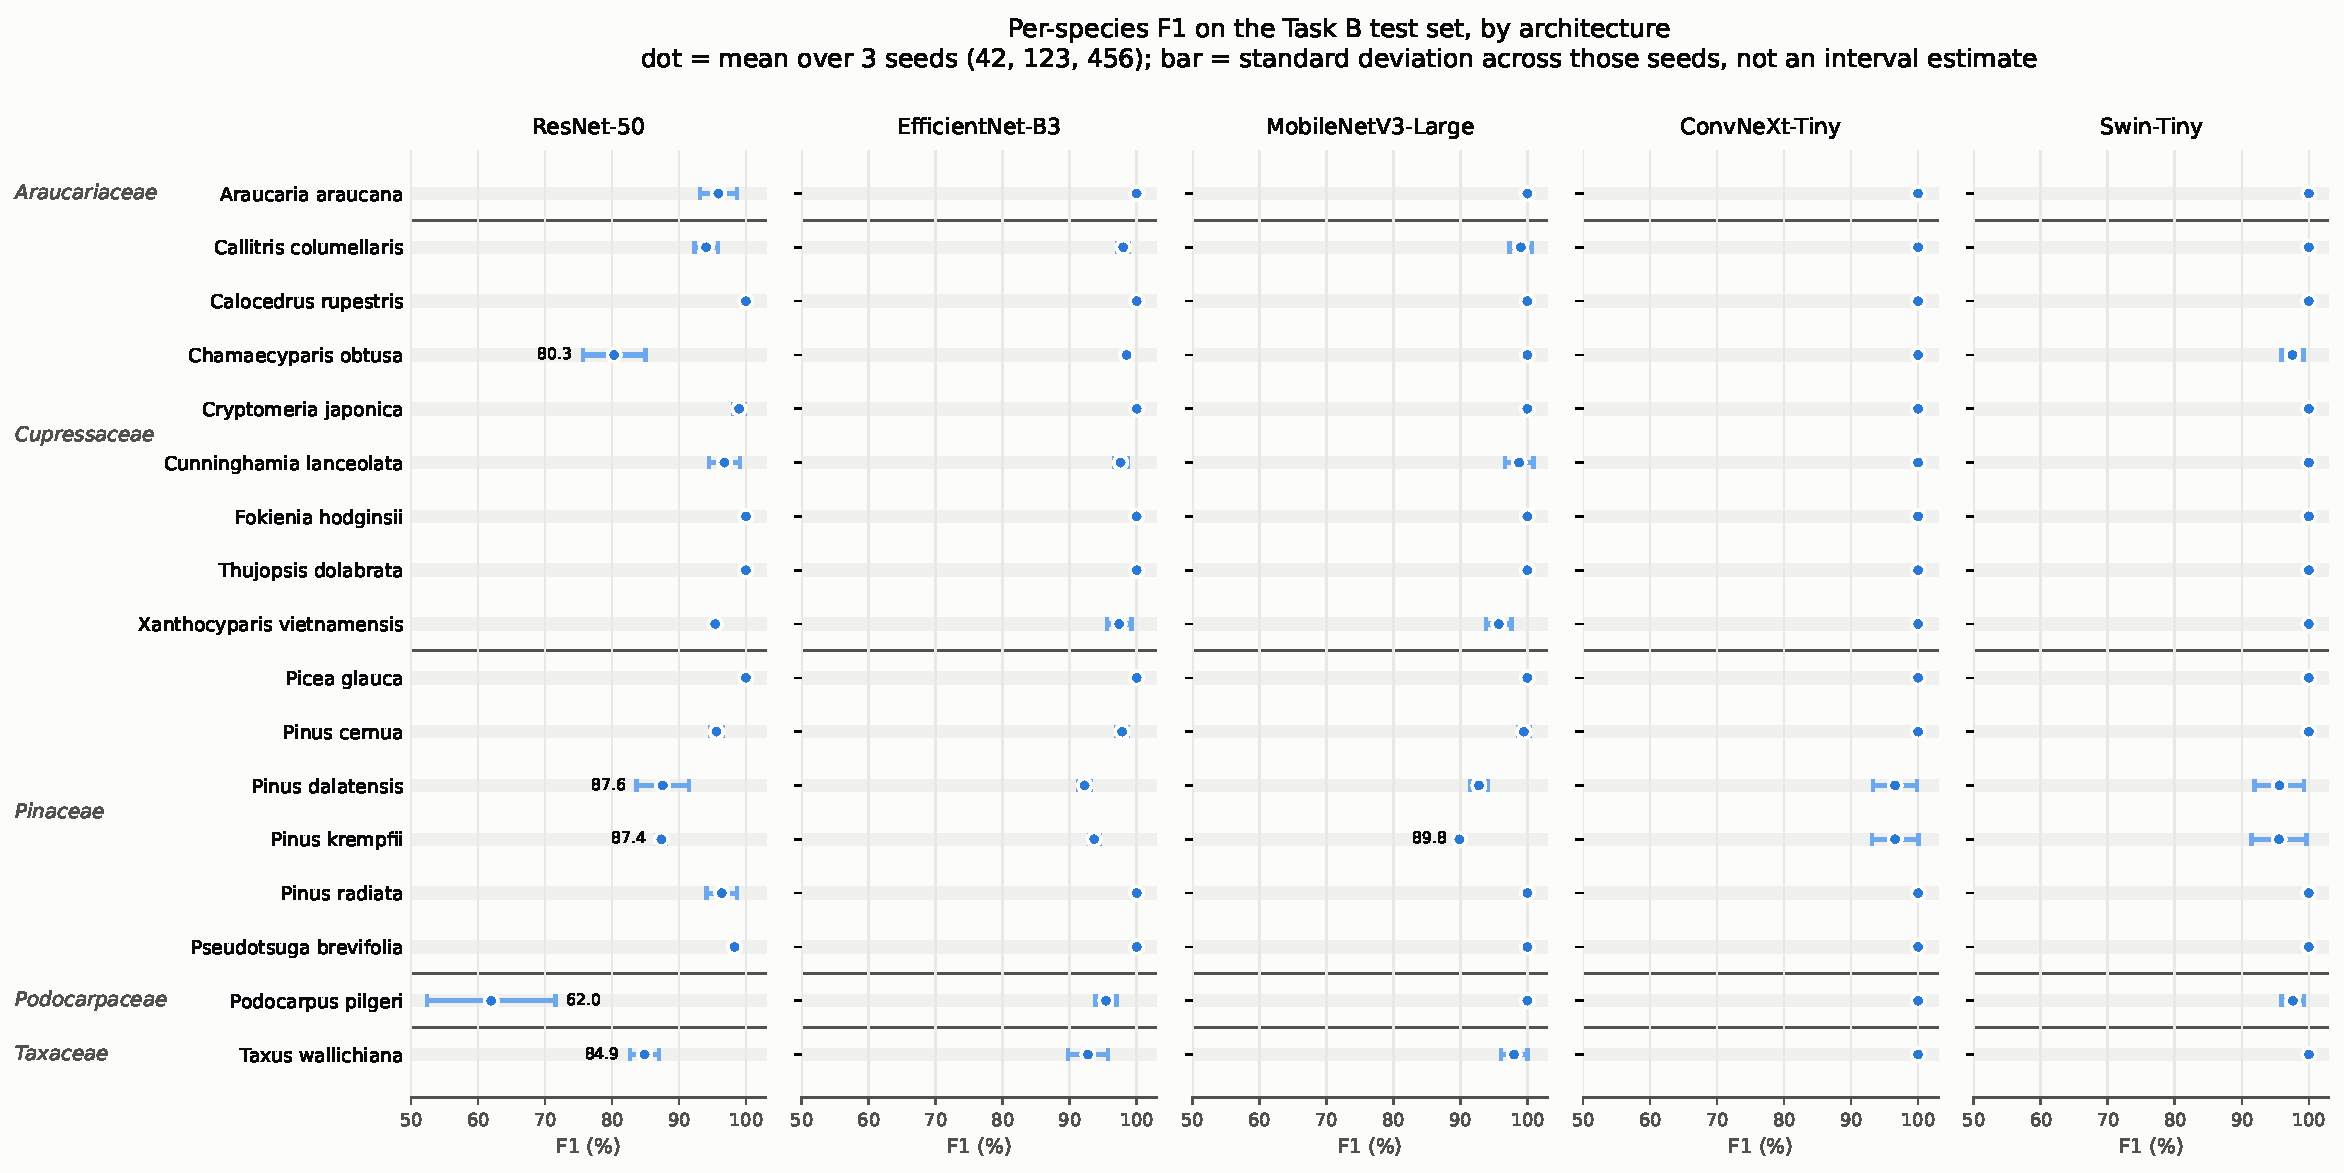
\includegraphics[width=\linewidth]{artifact/person3/per_class/fig_perclass_f1.pdf}
\caption{Điểm F1 theo từng loài trên tập test Task~B, mỗi panel một kiến trúc. Mỗi chấm là trung bình trên ba seed chính (42, 123, 456) và mỗi thanh là độ lệch chuẩn trên các seed đó; thanh này là thước đo phân tán trên ba lần chạy, không phải ước lượng khoảng. Các loài được sắp theo họ, các khối họ tách nhau bằng đường kẻ ngang và được ghi nhãn ở lề trái. Trục ngang mã hóa bằng vị trí nên không bắt đầu từ không; các giá trị dưới 90\,\% được ghi nhãn trực tiếp. Các kiến trúc được tách thành panel riêng thay vì phân biệt bằng màu, để danh tính được mang bởi vị trí và tiêu đề panel.}
\label{fig:perclass}
\end{figure}
